\hyperref[sec:sec25]{\section{為什麼香港到現在還未有普選?}}
\label{sec:sec34}

按人大常委二零零七的決定,香港本來最早可以二零一七年實施行政長官普選,之後可實施立法會普選。不過,由於二零一四/一五年的政改方案未獲通過,行政長官和立法會至今仍然沿用二零一二年的選舉模式,普選遙遙無期。要理解香港實現普選之難,得先回顧特區成立以來各次政改所遇到的波折。

香港的普選議題相對於其他地方的民主化有幾個明顯特點。首先,香港選舉政治的歷程較短,從區議會成立起算的話只有三十多年歷史。而在這過程中,選舉制度本身經常因政治環境而改變。例如在一九九一年至一九九八年期間,立法機關的三次選舉就用了三種不同的地方直選制度(雙議席雙票、單議席單票、比例代表制)。選舉制度缺乏時間鞏固和建立傳承,既有共識很容易被打破,近年接連出現參選人因政治因素被拒成為候選人就是一例,以至連怎樣的選舉才算是普選也可以成為爭議。

第二,香港的普選和民主化十分不平均,而且由外在力量決定。很多國家的民主化都涉及當地專制政府的倒台,及後各級議會便會同時民主化。在香港,民主化的步伐先由英國政府,繼而再由中國政府決定。就算香港人出盡全力向香港政府施加壓力,對中國政府的實際影響仍相當有限。如是者,香港的普選和民主化就很大程度上受限於中國政府的政治選擇;它可以一方面取消區議會的委任制,又把市政局和區域市政局撤除,對立法會和行政長官的選舉制度則寸步不讓。

不過,中國政府對香港的普選和民主化未至於可以完全任意妄為。首先,香港作為一個商港的歷史和角色,使得法治和法律程序的正當運用被視為金科玉律。這點使得公權力的運用和制度的變遷不能過於隨意,因而保障了公民自由在香港受到一定程度的保障。不過香港在缺乏民主管治的同時強調言論和新聞自由,就形成很大的內在矛盾。

香港的普選和民主化和其他地方還有一個很重要的分別:《基本法》列明香港最終會實施普選。換言之,《基本法》確立了香港目前的制度只應是暫時性的,而且不符合普選的定義,在恰當的時候是要改變的。相對來說,一些專制國家可以聲稱自己已經很民主,或聲稱已經以恰當的方式實現了民主的說法,在香港就不管用。香港人可以按《基本法》義正辭嚴的申明普選是一個承諾,他們爭取普選只是拿回本來應得的權利。當然,反過來說,《基本法》並沒有明文定義所述的普選其實是指什麼,而考慮到《基本法》的最終解釋權在於人大常委,香港的普選和民主化就要面對一個無法迴避的問題:人大常委所理解的普選,和香港人所爭取的普選,兩者所指未必相等,而這個困難正正體現在過去十多年來多次的政治改革爭議當中。

香港實施普選的憲制基礎載於《基本法》第四十五條第二款「行政長官的產生辦法根據香港特別行政區的實際情況和循序漸進的原則而規定,最終達至由一個有廣泛代表性的提名委員會按民主程序提名後普選產生的目標」和第六十八條第三款「立法會的產生辦法根據香港特別行政區的實際情況和循序漸進的原則而規定,最終達至全部議員由普選產生的目標」。至於這「雙普選」的啟動程序,則載於附件一第七項「二零零七年以後各任行政長官的產生辦法如需修改,須經立法會全體議員三分之二多數通過,行政長官同意,並報全國人民代表大會常務委員會批准」和附件二第三項「二零零七年以後香港特別行政區立法會的產生辦法和法案、議案的表決程序,如需對本附件的規定進行修改,須經立法會全體議員三分之二多數通過,行政長官同意,並報全國人民代表大會常務委員會備案」。

回到特區成立初期的理解,普遍認為二零零七年的行政長官選舉和二零零八年的立法會選舉,就是香港最早可以實施「雙普選」的時機。對於行政長官普選的方案,應順序經過三個關卡,即立法會、行政長官和人大常委;至於立法會的普選方案,則只要順序經過兩個關卡,即立法會和行政長官,人大常委只作備案。

人大常委於二零零四年四月六日就上述附件的解釋,推翻了這個普遍理解。該解釋所斟酌的字眼,在於條文中「如需修改」這四個字。人大常委的解釋把四個字擴展為「是否需要進行修改,香港特別行政區行政長官應向全國人民代表大會常務委員會提出報告,由全國人民代表大會常務委員會依照《中華人民共和國香港特別行政區基本法》第四十五條和第六十八條規定,根據香港特別行政區的實際情況和循序漸進的原則確定。修改行政長官產生辦法和立法會產生辦法及立法會法案、議案表決程序的法案及其修正案,應由香港特別行政區政府向立法會提出」。

這個解釋帶來了兩個新增的限制。第一,所謂「如需修改」的意思是可以修改也可以不修改,而是否有需要則是人大常委說了算,香港本身的內部共識不能作準。對於行政長官選舉來說,本來三步走的理解就變成了「五步曲」,加多了行政長官報告和人大常委回覆這兩個步驟,當中人大常委的角色除了最後批准外,還有對整個過程本身的啟動作出批准。對於立法會選舉,改變則更為翻天覆地:人大常委從原來沒有否決權,變成尚未開始就可以決定終止。第二,具體方案的提出權被特區政府所壟斷。原來的條文並沒有否定立法會議員自行提出方案,通過後才交由行政長官審批的可能性。經人大常委的解釋後,政改方案必定要由政府提出,免除立法會通過一個行政長官未必想接受的方案的可能。

\begin{figure}[htbp]
    \centering
    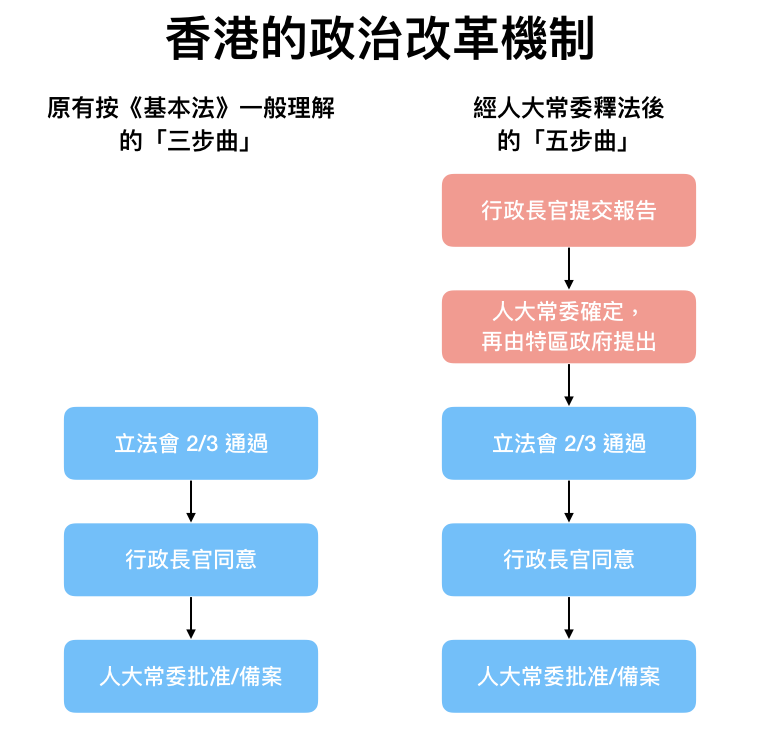
\includegraphics[width=0.7\textwidth]{c34/h-klesson1-056.png}
    \caption{由三步曲變成五步曲的政改機制} 
\end{figure}

按照人大常委的解釋,時任行政長官董建華於四月十五日向人大常委提交報告,認為二零零七年行政長官和二零零八年立法會的產生辦法應予以修改,報請人大常委確定是否可以修改。

就此,人大常委於四月二十六日作出回覆。注意董建華在報告中只是簡單詢問了產生辦法「是否可以修改」,但人大常委的回覆卻複雜得多:行政長官和立法會的產生辦法只可在兩個前提下作出修改。這些前提包括二零零七年行政長官和二零零八年立法會的選舉不實行普選,而立法會功能團體和分區直選產生的議員各佔半數的比例維持不變。至此,人大常委的角色又再一次擴展,從事先決定可否修改變成事先決定修改的範圍為何。更奇怪的,是董建華的報告並沒有問及立法會的表決程序可否修改,但人大常委卻回答了這條沒有問的問題,決定表決程序維持不變。如前文所述,「分組點票」正正是破壞香港議會文化的其中一個根源,人大常委的回覆卻把改革這個制度的路封死(見\hyperref[sec:sec21]{問題二十一})。

經此一役,香港政治改革的機制已明顯地和原來的理解相距很遠,中國政府可以完全限制香港民主化的時程和空間。自此以後,每隔數年香港就會經歷一次政改爭議:中國政府會訂下該次政改的框架,然後香港社會為是否接受這個框架爭執不休。

就二零零七年行政長官和二零零八年立法會的產生辦法,繼任董建華為行政長官的曾蔭權於二零零五年十月在人大常委的框架下提出方案。行政長官方面,建議選舉委員會從八百人增加至一千六百人,當中多數新增席位交予全體區議員出任。立法會方面,建議議席從六十席增加至七十席,其中五席為地區直選,另外五席則把功能界別中的的區議會界別由一席增至五席。

對此方案,民間出現兩種意見。贊成的意見認為在二零零七/零八年的選舉邁出踏向普選的第一步,有助與中央政府建立良性互動,十分重要。反對的意見則指出方案不包括立即取消區議會委任制,會衍生出由行政長官委任的區議員可直接在下一屆的行政長官選舉中投票的怪現象,為爭取連任者製造種票機會。新增立法會的區議會界別議席也沒有說明選舉方式,如以全票制選出的話便會全被送給建制陣營。此外,不少意見認為這一步走得太少,缺乏誠意,在沒有普選路線圖和時間表的前題下,不能接受。在非建制陣營團結反對下,該方案於二零零五年十二月在立法會因未得全體三分二議員支持而被否決。

普選路線圖和時間的問題,在下一次的政改諮詢中得到處理。二零零七年十二月,曾蔭權向人大常委提交報告,當中列明香港社會普遍希望能早日訂出普選時間表,為香港的政制發展定出方向。數日後,人大常委回覆行政長官最早可於二零一七年普選產生,之後立法會也可普選產生。二零一二年的行政長官和立法會則不以普選產生,而立法會的功能界別和地區直選的比例維持各半。

到了二零一零年四月,特區政府提出方案,內容與上次否決的版本大同小異,唯確立了政府會在通過方案之後提出取消區議會委任制。加上早前訂立的普選路線圖和時間表,上次觸發否決的三個主因已有兩個被解決。至於新增區議會界別議席的選舉方式,民主黨提議交由本來在功能界別沒有投票權的選民選出,此建議經一輪爭拗後終獲中央政府接受。而非建制陣營方面,則出現應該接受先走一步還是堅持沒有清晰普選方案便寧願否決的爭議。方案最終在民主黨和民協的支持下獲得立法會全體三分二議員支持而通過。儘管政改終於首次獲得通過,非建制陣營卻因此奉上嚴重分裂的代價。

當時除了民主黨和民協之外,也有不少學者和評論人認為應該讓方案通過。他們認為雖然方案未如理想,但仍希望透過通過方案來與中央政府建立良性互動,為將來二零一七年普選行政長官創造有利條件。很不幸,這個願望在二零一四年被人大常委的「八三一決定」所打破,引發的震撼直接導致佔領運動的發生。而在相關的政改方案被否決後,除非「八三一決定」有所改變,否則在可見將來要實現普選恐怕遙遙無期。

「八三一決定」是指中央政府對香港普選方案作出的具體規限。自從人大常委決定香港最早可於二零一七年實施普選後,各界隨即開始討論具體落實的方案。《基本法》第四十五條規定「行政長官的產生辦法根據香港特別行政區的實際情況和循序漸進的原則而規定,最終達至由一個有廣泛代表性的提名委員會按民主程序提名後普選產生的目標」,當中「提名委員會」和「按民主程序提名」成為爭議的焦點。畢竟,現時政府施政不暢的其中一個主因,是由於行政長官由選舉委會員選出,而選舉委會員本身不能代表民意(見問題十八)。爭取普選的其中一個主因,就是要解決由此而來的管治認授問題。因此,如果日後的提名委員會同樣不能代表民意,卻可限制誰能獲得提名,則選出的行政長官仍然要面對管治認授的挑戰,所謂的「普選」就只會徒具形式,卻不能解決實際問題。

要解決此困難,可有兩種解決方法。第一種是確保提名委員會的代表性,例如由立法會擔當提名委員會的角色,只要有數名議員聯署即可成為行政長官候選人。不過無論是坊間提出的方案(如陳弘毅方案、香港2020方案和18學者方案),或是特區政府向中央政府提交的報告,都傾向提名委員會沿用既有選舉委員會的方式產生,或只作小幅修改。

第二種進路,則是放棄把提名委員會民主化,而直接要求在提名委員會以外另立提名機制,提名委員會必須確認出線者為正式候選人。由多個非建制派政黨和團體成立的真普選普盟所提出的方案,即要求在提名委員會提名外,另立政黨提名(於最近一次立法會選舉中,獲得直選部分全香港總有效票數百分之五或以上的政黨或政治團體,單獨或聯合提名一名參選人)和公民提名(獲得百分之一登記選民具名聯署提名)。對此,政府表明任何其他推薦手法都不得妨礙提名委員會行使唯一實質的提名權。

按「五步曲」的要求,特區政府於二零一四年七月向中央政府提交報告,而人大常委則在八月三十一日就二零一六年的立法會選舉和二零一七年的行政長官選舉作出決定,也就是所謂的「八三一決定」。值得注意的,是按照過往的做法,人大常委在這一階段極其量只會說明哪一部分的選舉辦法需要修改,哪一部分則不需要修改。然而這次決定卻再進一步,直接規定了選舉辦法應該如何修改。按決定所述,提名委員會的人數、構成和委員產生辦法應按照上一屆的選舉委員會來規定,再由他們產生二至三名行政長官候選人,每名候選人均須獲得提名委員會全體委員半數以上的支持。全港選民只可以在這些獲提名的候選人之間作出選擇,而選出後的當選人要再由中央政府任命。

「八三一決定」的問題,在於從公眾參與的角度來說,在此框架下產生的方案都不可能比之前更為民主,甚至會有所倒退。普選的原意是要把選出行政長官的權力從選舉委員會交回市民手中,框架下選舉委員會變成了提名委員會,而當選行政長官的其中一個要求是得到過半數提名委員會支持,也就是說原選舉委員會的權力沒有減少過。與此同時,過去參選者只要得到八分之一的選舉委會員成員提名即可能成正式候選人,即使與中央政府政見不同者也能以此身分在各正式場合發表政見公開辯論,但框架下提名門檻從八分之一提升到二分之一,日後就會排除了這個可能性。

站在中央政府的角度出發,二分之一的提名門檻可保證能夠成為正式候選人的參選者都是中央政府認可的人選。不過站在確保選舉能做到普及而平等的立場,現有選舉委會員作為特權階層的角色將會持續,他們和行政長官之間的利益關係將揮之不去,原來希望通過普選理順香港管治問題的願望落空。對此,香港不少輿講都認為「八三一決定」不合符香港的實際情況。畢竟,普選選出的行政長官仍然要由中央政府任命,也就是說普選從來都不會影響到中央政府對人選的否決權,香港輿論普遍接受如果中央拒絕任命選出的人選,到時大可以重新再選一次;畢竟現在的制度正正是這樣規定的。現有規定亦已明文禁止曾犯若干罪行(如叛逆罪)的人士參選,所以說要以提名委員會為國家安全把關的說法也於理不合,畢竟它並不是一個司法機關。以一個沒有民意認授的提名委員會去決定參選資格,結果只會增加香港政治的不可測和不穩定性,不乎香港作為一個現代化國際大都會的需要。

\begin{figure}[htbp]
    \centering
    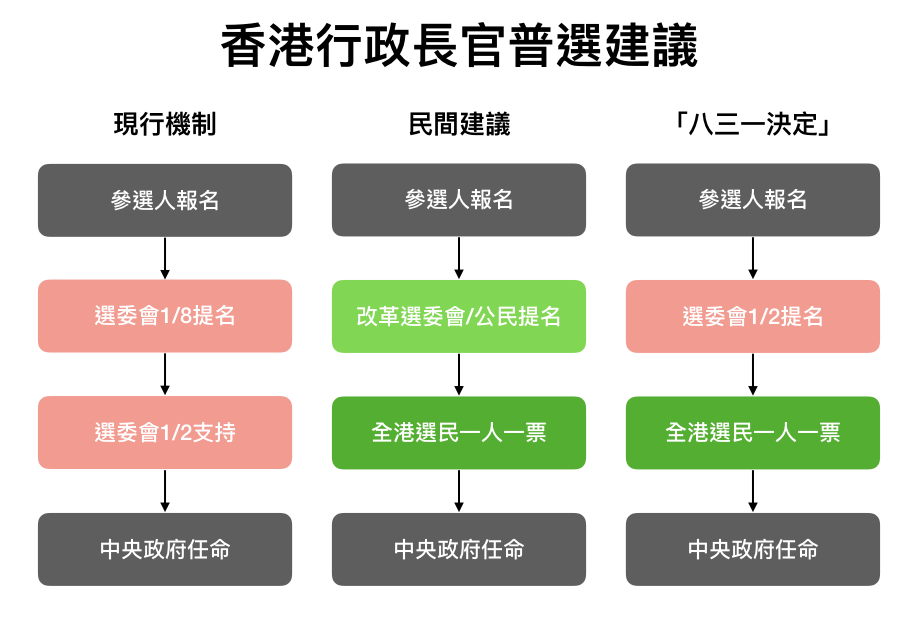
\includegraphics[width=0.7\textwidth]{c34/h-klesson1-057.png}
    \caption{「八三一決定」沒有解決選委會認授不足帶來的問題}
\end{figure}

「八三一決定」直接觸發了大專學界於九月中旬發動罷課,並最終演變成持續七十九日的佔領運動。儘管佔領運動未能迫使中央政府收回決定,但在巨大的民意壓力下非建制陣營也就團結一致將之否決。但這並不代表普選爭議就此便會告終。香港人爭取普選源於現在政治制度有結構性的缺陷,必須要通過實施普選來修正。當人大常委堵住了這個出路,香港人便只剩下兩個選擇:要求人大常委改變其決定,或索性尋求香港脫離人大常委的控制,也即是尋求香港獨立。

理論上,要解決普選爭議,還有一個可能的結局:非建制陣營失去在立法會三分之一的否決權,使得政府無論提出什麼樣的方案都會獲得通過,然後中央政府就可以聲稱香港已經達到《基本法》規定的普選目標。現實上,就算這事情真的發生,也不代表爭議就會真的告終。正如前文一直強調,普選是一個工具,目的是要解決管治問題。假普選就算被稱之為普選,也不會解決管治問題。民意的壓力就像是擠氣球一樣,壓緊一端的話便在另一端走出來;當權者固然也可以試試把每一端都困死,但結果只會是氣球爆開,同歸於盡。

\rule[-10pt]{15cm}{0.05em}

伸延閱讀:

Pun K (2008) The British legacy, \textit{The Political Future of Hong Kong} p1-25

Chan SCK (2015) Delay no more: struggles to re-imagine Hong Kong (for the next 30 years), \textit{Inter-Asia Cultural Studies} 16:3, 327–347.